\documentclass{article}
\usepackage{amsmath}
\usepackage{tikz}
\usepackage{geometry}
\usepackage{enumerate}
%\renewcommand{\labelenumi}{(\alph{enumi})}
%\renewcommand{\labelenumii}{(\roman{enumii})}
\usepackage{color}
\definecolor{Yellow}{rgb}{1,1,0}
\newcommand{\edit}[1]{\colorbox{Yellow}{#1}}


\geometry{verbose,letterpaper,tmargin=2cm,bmargin=2cm,lmargin=2cm,rmargin=2cm}

\title{CS181: MDPs and Reinforcement Learning}
\author{Danny Zhu \& Tianhui Cai}
\let\b\mathbf

\begin{document}
\maketitle
\begin{enumerate}
\item 
  \begin{enumerate}
  \item \emph{Given a probability distribution and utility function,
    write equations showing how to determine the optimal action, given
    the current score.}

    Let $U(s')$ be the utility function and $P(s'|s,a)$ the
    probability of going to $s'$ from $s$, given action $a$. Then the
    optimal action is $\pi(s,U,P)=\arg\max_{a\in A} \sum
    U(s')P(s'|s,a)$.

%  Let $A$ denote the set of places on the target to aim for. 
%  Let $a$ denote some action in $A$ and $s$ denote your current score. 
%  Then let $Q(s,a)=R(s,a)+\sum_{s'}P(s'|s,a) B(s')$
%  where $U(s,a)$ is the utility function and $B(s')$ is the
%  best score possibly obtained with $s'$ as a current score. 
%  $B(s')$ can be obtained through expectimax or value iteration. 
%  The best action to take with $s$ as a current score is 
%  $\pi^*(s)=\argmax_{a\in A} Q(s,a)$. 

  \item \emph{One of your colleagues proposes the following utility
    function:}
    \begin{align*}
      U(points,score)=
      \begin{cases}
        points & \text{ if } points \leq score\\
        0 & \text{ otherwise}
      \end{cases}
    \end{align*}
    \emph{In other words, the utility is equivalent to your change in
      score. What do you think of this proposal? If a dart player is
      designed using this proposal, what decisions would you expect it
      to make well, and what decisions would you expect it to make
      poorly?}

    This proposal is myopic. It would work well if lower point values
    were at least as easily obtained as larger ones. However, this may
    not be the case, i.e. if you started out with 10 points, and you
    could hit 5 and 9 with high probability, but 1 with extremely low
    probability, then it is better to aim for 5 and 5 rather than use
    the proposal which would suggest 9 and 1.
  \end{enumerate}

\item
  \begin{enumerate}
  \item \emph{What are the states and actions of your MDP model?
    Complete the \texttt{get\_states()} function in
    \texttt{darts.py}. (you may use the \texttt{test\_get\_states}
    unit test at this point)}

    The states are integers from 0 to 301. The actions are aiming for
    a particular section on the dartboard.

  \item \emph{Define the reward function: what reward or punishment do
    you receive for each state and action? What role does the discount
    factor play? Once you have specified this function, complete the
    reward function \texttt{R()} in \texttt{darts.py}. (see also the
    \texttt{test\_R} unit test).}

    Given a state $s$ and action $a$, if $s=0$, reward is 1; if $s\neq
    0$, reward is 0, since we win when we have a score of 0. This does
    not depend on action.

    If the discount factor is 1, we weight all time periods
    equally. This is not so good because it would mean we didn't care
    whether we won early or late. If the discount factor is low, it
    means that we'd much rather win now than later, i.e. earlier
    winning is better than later. If the discount factor is 0, it
    means we don't care at all about future winning, which is bad,
    since we will then only act nontrivially if we are one step away
    from winning.

    %\edit{UNSURE, AND DATA DOES NOT AGERE}

    \setcounter{enumii}3
  \item \emph{We have implemented the infinite horizon value iteration
    algorithm in \texttt{mdp.py}. Why might we choose to use an
    infinite rather than finite horizon to find an optimal policy in
    the dartboards scenario?  You may now get your first results by
    running the \texttt{Warm-up} task.}

    The length of the game is unbounded, since we could, e.g., have
    one point left to go and we keep scoring more than 1 point. It
    therefore makes sense to use an infinite horizon, rather than
    choosing some bound on the future.

  \item \emph{Describe the intuition behind an optimal policy
    resulting from value iteration using the small game.}

    It seems like for the large part, the policy tries to throw a dart
    at the wedge that will produce exactly the score it needs to get
    to 0.  There are exceptions, though; when score is 7 or 8, it aims
    to get 2 or 3 instead of 7 or 8, since it is impossible to obtain
    a score of 7 or 8 in one throw. This seems to make sense for the
    smaller sums because if it can get to 0 in one hit, it will try
    to. The 2 and 3 are probably picked because it is relatively easy
    to get from a score of 6 to 0.

  \item \emph{Still referring to the small game, how does the optimal
    policy vary as you change the discount factor? What is common
    across optimal policies?}

    It appears that with varying $\gamma$, the policy for when score
    is between 1 and 6 is the same, with the exception of when
    $\gamma=0$, in which case the policy is 6 or each state
    (i.e. there is no differentiation between states because the mdp
    doesn't look ahead at all). The policy appears to be the same for
    other $\gamma$ not equal to 0.5, with the exception of when it is
    0.9 or 1.0, in which case it assigns targets that would have
    output values 1 and 1 for 7 and 8. This might be because, with
    less discounting, the strategy is more inclined to take a slower,
    more conservative route to 0.

    %\edit{these results don't match the above analysis}

    The following results (number of throws) were obtained, averaging
    5 runs for each row.

    \begin{tabular}{r|c c c}
      $\gamma$ & 1 game avg & 5 games avg & 10 games avg \\
      \hline
      0.1 & 4 & 3.24 & 4.34 \\
      0.5 & 4.2 & 4.56 & 5.36 \\
      0.9 & 5.8 & 4.76 & 5.6 \\
    \end{tabular}

    These results agree with the earlier analysis that too low
    $\gamma$ does not solve for fewer throws.
  \end{enumerate}

\item 
  \begin{enumerate}
  \item \emph{Prove that if policy iteration terminates with the
    policy $\pi^*$, $\pi^*$ is an optimal stationary policy.}

    This basically holds by definition. An optimal stationary policy
    is defined to be one that satisfies the Bellman equations, i.e
    $\pi$ such that $\pi(s)=\arg\max_{a} \left[R(s,a)+\gammma
      \sum_{s'} P(s'|s,a)V^{\pi}(s')\right]$.  Policy iteration
    terminates with $\pi$ if it does not change after an iteration,
    i.e.  $\pi(s)=\arg\max_a Q^\pi (s,a)=\arg\max_a
    \left[R(s,a)+\gammma \sum_{s'} P(s'|s,a)V^{\pi}(s')\right]$ which
    is exactly the condition above.

    %% Policy iteration consists of repeating the following: given a
    %% $\pi(s)$, convert it to a set of $V(s)$ that agrees with it, then
    %% take the argmax of $Q(s,a)=R(s,a)+\gamma \sum_{s'}
    %% P(s'|s,a)V(s')$. This step is basically the same as one step of
    %% value iteration, which converges to a unique fixed point,
    %% i.e. between different steps, $V$ necessarily changes unless we
    %% have reached the maximum.

    %% So if value iteration has $\pi^*$ as a stationary point, i.e. if
    %% we take the corresponding $V$, and through the step $\pi$ and
    %% hence $V$ doesn't change, then it must be optimal by convergence /
    %% optimality of value iteration, i.e. if some $V$ is not optimal, on
    %% one step of value iteration $V$ necessarily will change, so that
    %% $\pi$ necessarily changes on one step of policy iteration.

  \item \emph{Prove that if $\pi^1$ is the policy before a policy
    iteration phase, and $\pi^2$ is the policy after the phase, then
    for every state $s$, $V^{\pi^2}(s)\geq V^{\pi^1}(s)$. [Hint: first
      try to prove $V^{\pi^2}(\hat s)\geq V^{\pi^1}(\hat s)$ when the
      action is only improved in state $\hat s$. Then argue this
      property holds for all states.]}

    Let's call these policies $\pi$ and $\pi'$ for ease of notation
    (aka typing).  Then $\pi'(s)=\arg\max_a Q^\pi (s,a)$, so that by
    considering $V^\pi(s)=R(s,\pi(s))+\gamma
    \sum_{s'}P(s'|s,\i(s))V^\pi(s')$ and
    $Q^\pi(s,\pi'(s))=R(s,\pi'(s))+\gamma \sum_{s'} P(s'|s,\pi'(s))
    V^\pi(s')$, then we have $V^\pi(s)\leq Q^\pi(s,\pi'(s))$ by
    definition of argmax, as it is choosing the best next action
    $\pi'$.

    Now, we expand out $V^\pi(s)\leq Q^\pi(s,\pi'(s))$:
    \begin{align*}
      V^\pi(s) & \leq Q^\pi(s,\pi'(s)) \\
      & = R(s,\pi'(s))+\gamma \sum_{s'} P(s'|s,a)V^\pi(s') \\
      & \leq R(s,\pi'(s))+\gamma \sum_{s'} P(s'|s,a) Q^\pi(s,\pi'(s))\\
      & \ldots \\
      & = V^{\pi'}(s)
    \end{align*}
    by an expanded definition of $V^{\pi'}$. 

    %% Assume not, i.e. that $V^{\pi^2}(\hat s)<V^{\pi^1}(\hat s)$ for
    %% some $s$.  Given $\pi_1$, by definition $V_1:=V^{\pi^2}$ is such
    %% that $V_1(s)=R(s,\pi_1(s))+\gamma
    %% \sum_{s'}P(s'|s,\pi_1(s))V_1(s')$.  By definition of
    %% $V_2:=V^{\pi^2}$, $V_2(s)=\max_a \left[R(s,a)+\gamma
    %%   \sum_{s'}R(s'|s,a)V_1(s)\right]$.  Then the claim is that (for
    %% contradiction)
    %% \[\max_a \left[R(s,a)+\gamma \sum_{s'}R(s'|s,a)V_1(s)\right] < R(s,\pi_1(s))+\gamma \sum_{s'}P(s'|s,\pi_1(s))V_1(s')\]
    %% But this is impossible, because for $a$ we can just take $\pi(s)$
    %% to obtain an equality, a contradiction.

  \item \emph{Deduce that policy iteration always terminates with an
    optimal stationary policy.}
    
    There are a finite number of policies, and each iteration either
    produces the same policy (in which case we're done, and by part
    (a) it's optimal) or we get a policy (approximately) strictly
    better (approximately being, if we have a sensible ordering so we
    don't oscillate between policies), so that there are a finite
    number of steps to go through.
  \end{enumerate}

\item 
  \begin{enumerate}
  \item \emph{Implement two exploration / exploitation strategies for
    deciding how to act in each epoch based on the current result of
    value iterations: these should be different.  Run the next tasks
    and create a graph of relationship between performance and epoch
    size. How do these graphs compare for both strategies?}

    Strategy 1: explore with probability .2.

    \begin{center}
      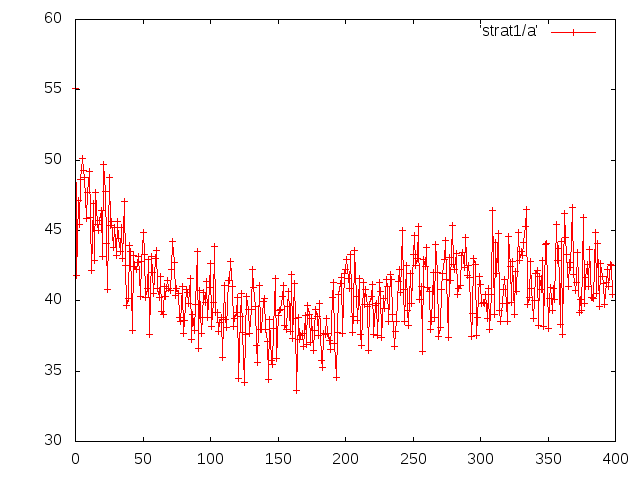
\includegraphics[scale=.4]{strat1.png}
    \end{center}

    For each epoch size, we plotted the average number of throws over
    250 games. The systematic change seems to be very small,
    especially compared to the random variation, but it looks like the
    number decreases up to an epoch size of about 150, then increases
    slightly again.

    Strategy 2: explore with probability (1/(iteration+5)).

    With this strategy, we had the interesting effect that many runs
    would end quickly, but many would take much, much longer. For
    example, 30 minutes of computation (running games in parallel)
    produced the following game lengths:
    \[16, 19, 20, 21, 21, 22, 22, 22, 24, 24, 24, 25, 29, 31, 33, 36, 43, 46, 48, 55, 557, 1622, 3134\]
    At that point, there were still many other trials that had not
    finished running yet, so the high end stretches up still further.

    \edit{Why does this happen?}

  \item \emph{Implement the model-free $Q$ learning algorithm as well
    as two exploration/ exploitation strategies that may be the same
    as in part (a). Pick a learning rate. Write code. Use the
    \texttt{Q-learning} task with the medium size game to compare the
    performance of your algorithm for both exploration / exploitation
    strategies.}

    Strategy 1: explore with probability .1.

    Strategy 2: explore with probability 100/(iteration+500).

    We chose $\alpha=.1$; running some trials indicated that it did
    not affect the performance noticeably. (That seems quite odd.) The
    first strategy almost always beats the second, with scores around
    22 compared to scores of around 30.

  \item \emph{Compare the performance of the model-based and
    model-free algorithms. Why do you think these algorithms performed
    relatively well or poorly?}

    The model-based algorithm seemed to perform much better. The
    system in use here is relatively simple and easily captured by a
    model, so that being able to incorporate the use of a model into
    the planning algorithm provides an advantage.

  \end{enumerate}

\end{enumerate}
\end{document}
